\section{Background} \label{sec:background}
To keep our discussion self-contained we only summarise the necessary mathematical details and notation required for our work. In this Section, we review the one-particle Green's function, the quantum singular-value transform algorithm and the single-impurity Anderson model that defines the physical system considered in our work.

\subsection{One-particle Green's Functions} \label{sec:G_functions}

The time-ordered single-particle Green's function (GF) at zero temperature in the frequency domain is defined in the Lehmann representation as \cite{lehmann1954eigenschaften, hjorth2017advanced}:
\begin{equation}
\label{eq:G_funct}
\begin{aligned}
    G_{ij}(z)  = G_{ij}^{(h)}(z) + G_{ij}^{(e)}(z),
\end{aligned}
\end{equation}
where:
\begin{subequations}
 \label{eq:GplusandGminus}
    \begin{equation}
    \label{eq:G_plus}
        \begin{aligned}
           G_{ij}^{(e)}(z) = \bra{\Psi_{0}} a_{i} \big( z - [H-E_{0}] \big)^{-1} a_{j}^{\dagger} \ket{\Psi_{0}},
        \end{aligned}
    \end{equation}
    %%
    \begin{equation}
    \label{eq:G_minus}
        \begin{aligned}
              G_{ij}^{(h)}(z) = \bra{\Psi_{0}} a_{j}^{\dagger} \big(z + [H-E_{0}] \big)^{-1}  a_{i}\ket{\Psi_{0}},
        \end{aligned}
    \end{equation}
\end{subequations}
For simplicity we have assumed $\ket{\Psi_{0}}$ to be non-degenerate, but this can be extended to degenerate ground-states at nonzero temperature. $G_{ij}^{(e)}(z)$ and $ G_{ij}^{(h)}(z)$ are called the advanced and retarded Green's function respectively, or the electron and hole excitation parts of the GF \cite{kosugi2020construction, tong2021fast}. Here $a_{i}$ and $ a_{i}^{\dagger}$ are fermionic creation and annihilation operators of an electron in the $i$-th spin orbital,  $\ket{\Psi_{0}}$ is the ground-state wavefunction, $E_{0}$ is the ground-state energy, $H$ is a  second quantized fermionic Hamiltonian and $z =\omega + i \delta$ is a complex frequency often interpreted as an energy shift \cite{tong2021fast}. The imaginary part of $z$, given by $\delta$, is small and required for convergence of the Fourier transform \cite{onida2002electronic}. Equation \ref{eq:G_funct} can be mapped to an equation involving qubit operators, by applying a fermionic-to-qubit transformation to the fermionic operators. For a given $z$, $G(z)\in \mathbb{C}^{N \times N}$ is an $N \times N$ matrix that is efficient to classically store, where $N$ is the number of spin orbitals (or qubits) describing the system. Equation \ref{eq:G_funct} shows how the $i$-th row and $j$-th column of $G(z)$ is calculated. Even though this matrix is efficient to store and manipulate classically, it should be noted that each entry requires solving an exponentially large problem. This is due to the size of the Hamiltonian scaling as $H \in \mathbb{C}^{2^{N} \times 2^{N}}$ or exponentially with the number of spin orbitals. Classically computing each entry in the Green's function quickly becomes intractable, as doing so requires inverting an exponentially large matrix. Such a Hilbert space is naturally expressed on a quantum computer with $N$ qubits. All that is  required is the ability to perform a matrix inverse on such a device. One way to do this is using the quantum singular-value transform algorithm. As will be discussed in the next section, this method provides a way to apply an (approximate) inverse of a block encoded operator onto a quantum state. %We note this approach does not give a user access to the singular-values or access to the inverted matrix. Algebrically 

% However, the quantum singular-value transform algorithm offers a way to calculate the matrix inverse on a quantum computer. 

A point to note when calculating the Green's function is that the ground-state $\ket{\Psi_{0}}$ must be known. In this work we assume it is known \textit{a priori} and can be efficiently prepared on a quantum device. However, in general the ground-state problem of a $l$-local Hamiltonian is QMA-complete for $l\geq 2$ (for $l=1$ the problem is in P) \cite{kempe2006complexity} and currently there are no known algorithms that can find a solution in polynomial time. How to find $\ket{\Psi_{0}}$ thus remains an open question and we do not consider this issue in the study presented here, as the toy system studied is classically tractable.

\subsection{Quantum Singular-Value Transform algorithm} \label{sec:QSVT_background}

A comprehensive review on quantum signal processing \cite{low2019hamiltonian} and the quantum singular-value transform \cite{gilyen2019quantum} can be found in \cite{martyn2021grand}. In this section we summarise the steps required to perform matrix inversion via QSVT. The algorithm can be broken down into four major steps:
\begin{enumerate}
    % \item Build a quantum circuit to prepre the ground-state ($\ket{\Psi_{0}}$).
    \item Construct a quantum circuit that block encodes a matrix.
    \item Generate the quantum signal-processing angles required to implement the desired function that will be applied to the singular values of the block encoded matrix. Here this will be an approximation of the inverse function: $f(x) \approx 1/x$.
    \item Construct the quantum circuit to implement the QSVT algorithm using the outputs of steps $1$ and $2$.
    \item Implement a Hadamard test to evaluate the real and complex parts of each entry in the Green's function.
\end{enumerate}
The following subsections review each of these steps, apart from the Hadamard test, which we did not implement in this work. A full analysis of step $4$ is given by Tong \textit{et al.} in \cite{tong2021fast}. %We assume the 1st step has been solved. This can be done through NISQ methods such as running VQE and also more fault tolerent procedures such as QPE. TODO maybe add imaginary time evolution.


\subsubsection{Linear Combination of Unitaries (block encoding)} \label{sec:block}

There are many different methods to block encode a matrix \cite{camps2022explicit, low2019hamiltonian}. In this paper, we focus on the linear combination of unitaries (LCU) approach, a technique to block encode any linear combinations of unitary operators \cite{childs2012hamiltonian, berry2015simulating}. Given such a matrix $A$:

\begin{equation}
 \label{eqn:A_def}
\begin{aligned}
	A &= \sum_{i=0}^{k-1} \alpha_{i} U_{i}, \text{ where} \\
 \| A\| &\leq \sum_{i=0}^{k-1} \bigg( |\alpha_{i}| \cdot \underbrace{\| U_{i}\|}_{=1} \bigg) = \sum_{i=0}^{k-1} |\alpha_{i}| = \|A \|_{1},
	\end{aligned}
\end{equation}
where, without loss of generality, we can assume $\alpha_{i}>0$ and $\alpha_{i} \in \mathbb{R}$ $\forall i$ by absorbing any complex phases and signs into the unitaries  $U_{j}$ \cite{childs2012hamiltonian, low2019hamiltonian, ralli2021implementation}.  Given a list of $\alpha_{i}$ and each $U_{i}$, which are assumed to be easy to implement as controlled operations on a quantum device, the block encoding can be constructed using the oracles \cite{ low2019hamiltonian, ralli2021implementation}:

\begin{equation}
 \label{eqn:prep_oracle}
\begin{aligned}
	\prep &= \sum_{i=0}^{k-1} \sqrt{\frac{\alpha_{i}}{ \| A\|_{1}}} \ket{i}\bra{0}_{p}+ \hdots \\
 &= \begin{bmatrix}
\sqrt{\big(\frac{\alpha_{0}}{\|A\|_{1}}\big)} & \cdot & \hdots \\ 
\sqrt{\big(\frac{\alpha_{1}}{\|A\|_{1}}\big)} & \cdot & \hdots  \\ 
\vdots &  \ddots & \hdots   \\ 
\sqrt{\big(\frac{\alpha_{k-1}}{\|A\|_{1}}\big)} & \cdot  &  \hdots
\end{bmatrix},
	\end{aligned}
\end{equation}
and
\begin{equation}
 \label{eqn:select_oracle}
\begin{aligned}
	U_{\select} &= \sum_{i=0}^{k-1} \Big( \ket{i}\bra{i}_{p} \otimes U_{i} \Big).
	\end{aligned}
\end{equation}
Here the subscript $s$ denotes the system register and $p$ the $prep$ (ancilla) register.  The number of prep qubits required will be $n_{p}=\lceil \log_{2}(k)\rceil$, where $k$ is the number of unitaries in the LCU.

The $\prep$ or ``Prepare'' oracle  is a unitary that prepares the state  $\ket{P} = \sum_{i=0}^{k-1} \sqrt{\frac{\alpha_{i}}{\|A\|_{1}} }\ket{i}$ from the all zero state on the $prep$ register - i.e. $\ket{\bar{0}} \mapsto \ket{P}$.  This is why in equation \ref{eqn:prep_oracle} only the first column of the $\prep$ unitary is defined. As discussed in \cite{ralli2021implementation}, the other columns can be take any value providing that $\prep$ remains unitary.  This means there is a lot of freedom in how to construct this operator. If one simply finds the quantum circuit that realises $\ket{\bar{0}}_{p} \mapsto \ket{P}_{p}$,  then the circuit's action on the other basis states are automatically accounted for and the whole of $\prep$ will be defined \cite{ralli2021implementation}. The only quantum circuit requirement is being able to generate any real quantum state from the all-zero state on the prep register. There are many different proposals on how to prepare arbitrary quantum states \cite{Long2001, Mottonen2005, Markov2006prep, Araujo2021}. Following the approaches given in both \cite{Markov2006prep, Araujo2021}, a real quantum state can be generated using multiplexed $R_{y}$ rotations with the number of single-qubit and CNOT gates both scaling as $\mathcal{O}(2^{n_{p}})$. As the number of $prep$ qubits scales logarithmically with the number of terms in $A$, $\mathcal{O}(\log_{2}|A|)$, the number of single-qubit and CNOT gates will scale linearly as $\mathcal{O}(|A|)$ for the $\prep$ part of the block-encoding circuit. 

The desired LCU block encoding is achieved by performing $\prep^{\dagger} U_{\select}\prep$ and post selecting on the all-zero state on the prep qubit register. We can check this via the following proof \cite{ low2019hamiltonian}:

% Figure environment removed

% The overall circuit produces the following final state $\big(\mathcal{I}^{prep} \ket{\bar{0}}^{prep} \otimes M \ket{\psi}^{sys} \big)+ \sqrt{ 1- \| M \ket{\psi}^{sys} \|^{2}} \ket{\perp}^{\substack{prep \\ sys}}$.  

\begin{equation}
\begin{aligned}
&\bigg[ \bra{\bar{0}}_{p} \otimes I_{s} \bigg] (\prep^{\dagger} \otimes I_{s} ) U_{\select} \big(   \prep \otimes I_{s}\big)\bigg[ \ket{\bar{0}}_{p} \otimes I_{s} \bigg] \\
&=\bigg[ \bra{P}_{p} \otimes I_{s} \bigg] U_{\select} \bigg[ \ket{P}_{p} \otimes I_{s} \bigg] \\
&=  \bigg[ \bra{P}_{p} \otimes I_{s} \bigg] U_{\select} \Bigg( \underbrace{\sum_{i=0}^{k-1} \sqrt{\frac{\alpha_{i}}{\|A\|_{1}} }\ket{i}_{p}}_{\ket{P}_{p} }\otimes I_{s}  \Bigg) \\
 &=  \bigg[ \bra{P}_{p} \otimes I_{s} \bigg] \Bigg( \underbrace{ \sum_{i=0}^{k-1} \sqrt{\frac{\alpha_{i}}{\|A\|_{1}} }\ket{i}_{p}\otimes U_{i}}_{\text{equation \ref{eqn:select_oracle}}}  \Bigg) \\
	&= \Bigg( \sum_{j=0}^{k-1} \sqrt{\frac{\alpha_{j}}{\|A\|_{1}} }\bra{j}\otimes I_{s}  \Bigg) \Bigg( \sum_{i=0}^{k-1} \sqrt{\frac{\alpha_{i}}{\|A\|_{1}} }\ket{i}_{p} \otimes U_{i}  \Bigg) \\
	&= \sum_{j=0}^{k-1}\sum_{i=0}^{k-1} \frac{\sqrt{\alpha_{i}\alpha_{j}}}{\|A\|_{1}} \bra{j} i \rangle_{p} \otimes U_{i} \\
	&= \frac{1}{\|A\|_{1}} \sum_{i=0}^{k-1} \alpha_{i} U_{i}.
	\end{aligned}
\end{equation}
This is implemented according to the circuit in Figure \ref{fig:block_encode_circ}. The probability of success for this block encoding is $(\|A\|_{1})^{-2}\bra{\psi}_{s} A^{\dagger} A \ket{\psi}_{s}$. As discussed in \cite{ralli2021implementation}, $A$ is not necessarily unitary and so $A^{\dagger}A$ may not equal $I$. The probability of success therefore depends on the system state $\ket{\psi}$ and the $1$-norm of the block-encoded matrix. Amplitude amplification  \cite{grover1998quantum, brassard2002quantum, yoder2014fixed} and oblivious amplitude amplification \cite{berry2014exponential, yan2022fixed} can then be used to increase the probability of success \cite{gilyen2019quantum}.

In the literature, it is common to see  $(\alpha, \kappa, \epsilon)$-block encodings. Here $\alpha$ is a normalisation factor of the block-encoded matrix, $\kappa$ is the number of extra ancillary qubits required to implement the block encoding and $\epsilon$ is the error of the block encoding. 

In this work, the LCU is given as a linear combination of Pauli operators. The ``$\select$'' oracle (equation \ref{eqn:select_oracle}) applies a controlled version of each of these Pauli operators on the system register, controlled by the prep register. This requires performing multi-control Pauli operators with phases $\{ i,-i,1,-1 \}$. Following the work in \cite{ralli2021implementation}, this can achieved using the template given in Figure \ref{fig:cntrl_P_gate}. The relevant phases are then obtained via the following identities:

\begin{subequations}
 \label{eq:pauli_phases}
    \begin{equation}
    \label{eq:neg_sign}
	-Z =XZX,
    \end{equation}
    %%
\begin{equation}
    \label{eq:imag}
R_{z}(\mp \pi)= e^{\mp i \frac{\pi}{2}Z}  = \pm i Z.
\end{equation}
\end{subequations}
These can be implemented according to the circuit templates summarised in Figure \ref{fig:phaseZgates}. By performing a change of basis on certain qubits, using the single-qubit gates $\{S, S^{\dagger}, H \}$, the circuit proposed in Figure \ref{fig:cntrl_P_gate} can be used to generate any multicontrol Pauli operator with a $\pm 1, \pm i$ phase. We note the ordering of unitaries in   equation \ref{eqn:select_oracle} is arbitrary, but an optimal ordering can lead to significant circuit simplifications. We leave this as an open question, but note the work in \cite{ralli2021implementation}, \cite{hastings2014improving} and \cite{cowtan2019phase} can readily be applied to this problem.  

 % If this construction is decomposed into $CNOT$ and $U3$ gates, then $4 n^{2} - 4 n + 2$  $CNOT$ and $4 n^{2} - 2$ $U3$ gates are required.


To determine the overall circuit cost to implement  $U_{\select}$ (equation \ref{eqn:select_oracle} and Figure \ref{fig:block_encode_circ}), we need to determine the cost of implementing a multicontrol $Z$ gate and multicontrol $R_{z}$ gate. Following the proposal by da Silva and Park, any $n$-control single-qubit gate can be decomposed with $\mathcal{O}(n^{2})$ single qubit and CNOT gates with linear depth \cite{da2022linear}. For an $n$-control single qubit $Z$ gate with $n \leq 6$, the approach outlined in \cite{bullock2003smaller} and  \cite{shende2005synthesis} (theorem 8)  requires fewer two-qubit gates, where the number of single-qubit and CNOT gates required scales as $\mathcal{O}(2^{n})$ respectively. In general, using the work of da Silva and Park makes the cost of performing a multicontrol Pauli operator via the template in Figure  \ref{fig:cntrl_P_gate} scale as:
\begin{enumerate}
    \item $O(2n_{s})$ single-qubit gates, required to implement a change of basis.
    \item $O(2[n_{s}-1])$ CNOT gates, performing the ladder of CNOT gates on the system register.
    \item $O(n_{c}^{2})$ CNOT and single-qubit gates for the multicontrol $i^{k}Z$ gate.
\end{enumerate}
%$O(2n_{s})$ single qubit gates (required to implement a change of basis), $O(2[n_{s}-1])$ CNOT gates (representing the ladder of CNOT gates) and $O(n_{c}^{2})$ CNOT and single qubit gates for the multicontrol $i^{k}Z$ gate.
Here $n_{c}$ is the number of control qubits and $n_{s}$ is the number of `system' qubits the Pauli operator acts on. The single-qubit and CNOT gate cost per $n_{c}$-controlled Pauli operator scales linearly in system qubits and quadratically in control qubits as  $O(n_{c}^{2}+n_{s})$. The overall cost of implementing $U_{\select}$ via the circuits presented will depend on the number of $n_{c}$-controlled Pauli operators that are performed. Looking at Equation  \ref{eqn:select_oracle}, we see that $k$ operators are needed bringing the final cost to $O(k[n_{c}^{2}+n_{s}])$ single and two-qubit gates. As $k = |A|$ and $n_{c} = \lceil \log_{2}(|A|) \rceil$, we can write the final scaling  of single-qubit and CNOT gates as  $\mathcal{O}\Big( |A| ( \lceil \log_{2}(|A|) \rceil^{2} + n_{s} ) \Big)$. Table \ref{table:circuit_summary} provides a summary for the scaling of each part of the circuit.

 %\onecolumngrid
\begin{table*}[t]
\begin{adjustbox}{width=1\textwidth}
\begin{tabular}{llccl}
\hline
\hline
Citation              & Circuit / Gate                     & CNOT                                                         & Single                                                       & Comments                                                                                                                                                                                         \\
\hline
\hline
Shende \textit{et al.} \cite{Markov2006prep} & \begin{tabular}[c]{@{}l@{}} Circuit to prepare  any  \\ real amplitude $n$-qubit state \end{tabular} & $\mathcal{O}(2^{n})$                                         & $\mathcal{O}(2^{n})$                                         & \begin{tabular}[c]{@{}l@{}} Useful for $\prep$ part of LCU method, where $n=\lceil \log_{2}(|A|) \rceil$, \\ and thus $\mathcal{O}(2^{\log_{2}(|A|)}) =\mathcal{O}(|A|)$.  \end{tabular} \\

Silva and Park \cite{da2022linear}        & $n_{c}$-control $Z$                 & $\mathcal{O}(n_{c}^{2})$                                     & $\mathcal{O}(n_{c}^{2})$                                     & -                                                                                                                                                              \\
Bullock and Markov \cite{bullock2003smaller}    & $n_{c}$-control $Z$                 & $\mathcal{O}(2^{n_{c}})$                                      & $\mathcal{O}(2^{n_{c}})$                                          & For $n_{c}\leq 6$, requires fewer CNOT gates than Silva and Park approach. \\ \hline 
This work             & $n_{c}$-control $P$                 & $\mathcal{O}(n_{c}^{2}+ n_{s})$                              & $\mathcal{O}(n_{c}^{2} + n_{s})$                              & Circuit illustrated in Figure \ref{fig:cntrl_P_gate} up to single-qubit change of bases.                        \\ 
This work             & $\select$  &  $\mathcal{O}\Bigg( |A| \bigg( \lceil \log_{2}(|A|) \rceil^{2} + n_{s} \bigg) \Bigg)$ &$\mathcal{O}\Bigg( |A| \bigg( \lceil \log_{2}(|A|) \rceil^{2} + n_{s} \bigg) \Bigg)$ & \begin{tabular}[c]{@{}l@{}} \hline $U_{\select}$ circuit cost for a linear combination of $|A|$ Pauli \\  operators. Circuit template given in Figure \ref{fig:block_encode_circ}. \end{tabular}   \\                                                         \hline
\hline
\end{tabular}
\end{adjustbox}
\caption{Circuit scaling summary for different unitaries required to implement a block encoding of a linear combination of Pauli operators via the LCU method. Here $|A|$ denotes the number of Pauli operators in $A$ (Equation  \ref{eqn:A_def}), $n_{c}$ denotes the number of control qubits and $n_{s}$ denotes the number of system qubits.}
\label{table:circuit_summary}
\end{table*}
% \twocolumngrid
% 

% Figure environment removed

% Figure environment removed

The SIAM Hamiltonian considered in this paper is  constructed as a linear combination of Pauli operators  (equation \ref{eq:H_hubb}). Each individual Pauli operator $P_{i}$ is a unitary Hermitian operator that is easy to implement on a quantum computer as a controlled operation. However, rather than block encoding $H$, we  block encode the following complex shifted Hamiltonians:
\begin{subequations}
\label{eq:A_B}
    \begin{equation}
    \label{eq:A}
        \begin{aligned}
           B_{(e)} = \big( z - [H-E_{0}] \big)^{\dagger},
        \end{aligned}
    \end{equation}
    %%
    \begin{equation}
    \label{eq:B}
        \begin{aligned}
        C_{(h)} = \big( z + [H-E_{0}]\big)^{\dagger},
        \end{aligned}
    \end{equation}
\end{subequations}
The reason why the Hermitian conjugate is taken, in equations \ref{eq:A} and \ref{eq:B}, stems from how a matrix inverse can be obtained from a singular-value decomposition. If we write the  singular vector decomposition of an arbitrary matrix $A = U \Sigma V^{\dagger}$, then its inverse (if it exists) is $A^{-1} =  V \Sigma^{-1} U^{\dagger}$. Taking the Hermitian conjugate of $A$ yields $A^{\dagger} = V \Sigma  U^{\dagger}$ and to find the inverse of $A$ all that remains is to invert the singular values of $A^{\dagger}$.

The QSVT algorithm approximately inverts the singular values of a block encoded matrix. Performing this algorithm on the block encodings of $B_{(e)}$ and $C_{(h)}$ will therefore allow us to calculate the inverse parts of equations \ref{eq:G_plus} and \ref{eq:G_minus}. We calculate each inverse separately to reduce the circuit depth; however, it is possible to calculate the terms simultaneously using the method of adding different block encodings given in \cite{gilyen2019quantum, von2021quantum}. We decided not to implement this, as we wanted our approach to be more amenable to early fault-tolerant quantum computers.

As $z$ is a constant complex shift (has a real and imaginary component),  $B_{(e)}$ and $C_{(h)}$ are no longer Hermitian operators, whereas $H$ is. The Quantum Eigenvalue Transformation (QET) implements a polynomial transformation of a block-encoded Hermitian matrix when the polynomial of interest is represented by QSP \cite{low2019hamiltonian}. For a polynomial transformation of a general matrix the quantum singular-value transformation is used \cite{gilyen2019quantum}, hence why it is used in this work. We note that for a Hermitian matrix with a block-encoding input model, the quantum circuits of QET and QSVT can be the same \cite{dong2022ground}. Interestingly, it is possible to convert the non-Hermitian problem into a Hermitian one via matrix dilation, which requires an extra qubit - for further details  see Section 4.2 in \cite{chakraborty2018power}. This approach is unnecessary here, but the method of dilation is useful to know and we mention it in passing. This technique would be required if the quantum linear-system algorithm proposed by Harrow, Hassidim, and Lloyd (HHL) were to be used \cite{harrow2009quantum, cai2020quantum}.

Finally, we reiterate a comment made in \cite{martyn2021grand} on block encodings - much more work is necessary to find block encoding techniques specific to the relevant physical system. The LCU method is very general, but doesn't utilise any underlying structure of a problem and requires $\lceil \log_{2} (|A|) \rceil$ extra ancillary qubits. However, it is possible to make a $(\alpha,1,0)$ block encoding of any $n$-qubit matrix $A$ - i.e. only requiring a single ancilla qubit for a block encoding (see example 6.2 in \cite{lin2022lecture} and appendix D in \cite{lin2021real}). These schemes require a singular-value decomposition of $A$ and thus will not scale in a general setting. However, certain structures in particular physical problems may allow for more efficient encoding strategies. We leave this as an important open question.

%! \usetikzlibrary{decorations.pathreplacing,decorations.pathmorphing}
\providecommand{\ket}[1]{\left |#1\right\rangle}
\providecommand{\bra}[1]{\left\langle #1|\right}
\definecolor{mygreen}{RGB}{34,139,33}
\definecolor{myblue}{RGB}{157,220,229}
\definecolor{myred}{RGB}{255,99,98}
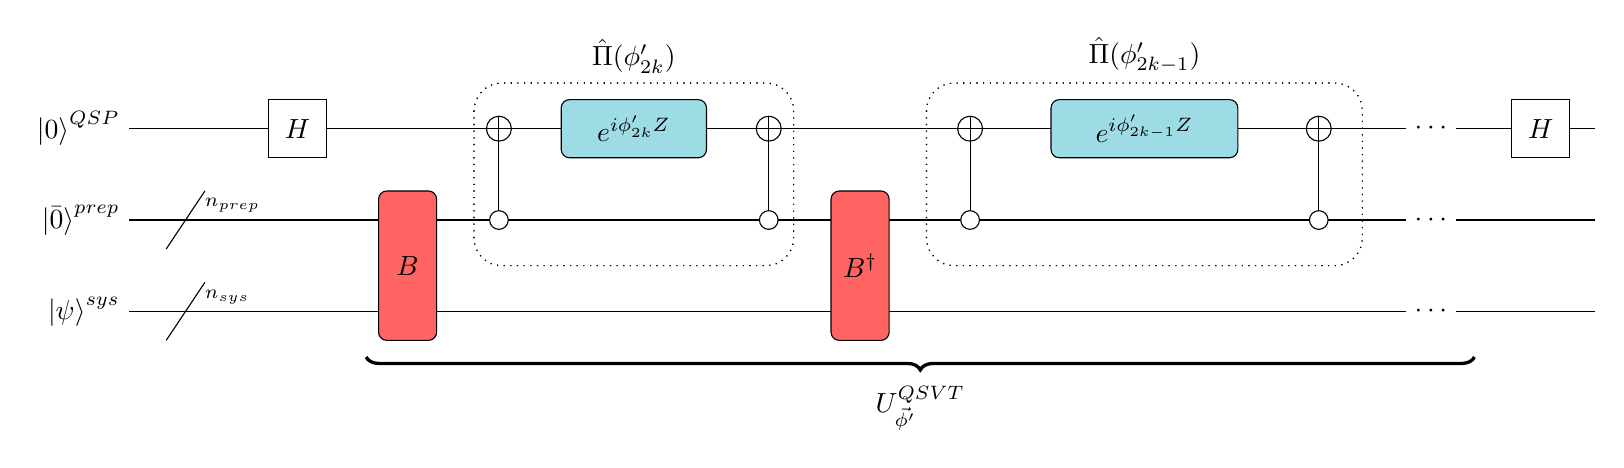
\begin{tikzpicture}[scale=1.500000,x=1pt,y=1pt]
\filldraw[color=white] (0.000000, -11.000000) rectangle (353.000000, 55.000000);
% Drawing wires
% Line 14: q0 W \ket{0}^{QSP}
\draw[color=black] (0.000000,44.000000) -- (353.000000,44.000000);
\draw[color=black] (0.000000,44.000000) node[left] {$\ket{0}^{QSP}$};
% Line 15: q1 W \ket{\bar{0}}^{prep}
\draw[color=black] (0.000000,22.000000) -- (353.000000,22.000000);
\draw[color=black] (0.000000,22.000000) node[left] {$\ket{\bar{0}}^{prep}$};
% Line 16: q2 W \ket{\psi}^{sys}
\draw[color=black] (0.000000,0.000000) -- (353.000000,0.000000);
\draw[color=black] (0.000000,0.000000) node[left] {$\ket{\psi}^{sys}$};
% Done with wires; drawing gates
% Line 18: q0 LABEL
% Line 19: q1 / n_{prep}
\draw (8.833333, 15.000000) -- (18.166667, 29.000000);
\draw (15.833333, 25.500000) node[right] {$\scriptstyle{n_{prep}}$};
% Line 20: q2 / n_{sys}
\draw (8.833333, -7.000000) -- (18.166667, 7.000000);
\draw (15.833333, 3.500000) node[right] {$\scriptstyle{n_{sys}}$};
% Line 23: q0 G $H$
\begin{scope}
\draw[fill=white] (40.500000, 44.000000) +(-45.000000:9.899495pt and 9.899495pt) -- +(45.000000:9.899495pt and 9.899495pt) -- +(135.000000:9.899495pt and 9.899495pt) -- +(225.000000:9.899495pt and 9.899495pt) -- cycle;
\clip (40.500000, 44.000000) +(-45.000000:9.899495pt and 9.899495pt) -- +(45.000000:9.899495pt and 9.899495pt) -- +(135.000000:9.899495pt and 9.899495pt) -- +(225.000000:9.899495pt and 9.899495pt) -- cycle;
\draw (40.500000, 44.000000) node {$H$};
\end{scope}
% Line 24: q1 LABEL
% Line 25: q2 LABEL
% Line 27: q1 q2 G:block $B$
\draw[rounded corners=3pt] (67.000000,22.000000) -- (67.000000,0.000000);
\begin{scope}[rounded corners=3pt]
\begin{scope}
\draw[fill=myred] (67.000000, 11.000000) +(-45.000000:9.899495pt and 25.455844pt) -- +(45.000000:9.899495pt and 25.455844pt) -- +(135.000000:9.899495pt and 25.455844pt) -- +(225.000000:9.899495pt and 25.455844pt) -- cycle;
\clip (67.000000, 11.000000) +(-45.000000:9.899495pt and 25.455844pt) -- +(45.000000:9.899495pt and 25.455844pt) -- +(135.000000:9.899495pt and 25.455844pt) -- +(225.000000:9.899495pt and 25.455844pt) -- cycle;
\draw (67.000000, 11.000000) node {$B$};
\end{scope}
\end{scope}
% Line 29: q0 C -q1
\draw (89.000000,44.000000) -- (89.000000,22.000000);
\begin{scope}
\draw[fill=white] (89.000000, 44.000000) circle(3.000000pt);
\clip (89.000000, 44.000000) circle(3.000000pt);
\draw (86.000000, 44.000000) -- (92.000000, 44.000000);
\draw (89.000000, 41.000000) -- (89.000000, 47.000000);
\end{scope}
\draw[fill=white] (89.000000, 22.000000) circle(2.250000pt);
% Line 30: q0 G:phase width=35  $e^{i\phi_{2k}'Z}$ % $\hat{\Pi}(\phi_{2k}')$
\draw (121.500000, 55.000000) node[text width=144pt,above,text centered] {$\hat{\Pi}(\phi_{2k}')$};
\begin{scope}[rounded corners=3pt]
\begin{scope}
\draw[fill=myblue] (121.500000, 44.000000) +(-45.000000:24.748737pt and 9.899495pt) -- +(45.000000:24.748737pt and 9.899495pt) -- +(135.000000:24.748737pt and 9.899495pt) -- +(225.000000:24.748737pt and 9.899495pt) -- cycle;
\clip (121.500000, 44.000000) +(-45.000000:24.748737pt and 9.899495pt) -- +(45.000000:24.748737pt and 9.899495pt) -- +(135.000000:24.748737pt and 9.899495pt) -- +(225.000000:24.748737pt and 9.899495pt) -- cycle;
\draw (121.500000, 44.000000) node {$e^{i\phi_{2k}'Z}$};
\end{scope}
\end{scope}
% Line 31: q0 C -q1
\draw (154.000000,44.000000) -- (154.000000,22.000000);
\begin{scope}
\draw[fill=white] (154.000000, 44.000000) circle(3.000000pt);
\clip (154.000000, 44.000000) circle(3.000000pt);
\draw (151.000000, 44.000000) -- (157.000000, 44.000000);
\draw (154.000000, 41.000000) -- (154.000000, 47.000000);
\end{scope}
\draw[fill=white] (154.000000, 22.000000) circle(2.250000pt);
% Line 33: q1 q2 G:block $B^{\dagger}$
\draw[rounded corners=3pt] (176.000000,22.000000) -- (176.000000,0.000000);
\begin{scope}[rounded corners=3pt]
\begin{scope}
\draw[fill=myred] (176.000000, 11.000000) +(-45.000000:9.899495pt and 25.455844pt) -- +(45.000000:9.899495pt and 25.455844pt) -- +(135.000000:9.899495pt and 25.455844pt) -- +(225.000000:9.899495pt and 25.455844pt) -- cycle;
\clip (176.000000, 11.000000) +(-45.000000:9.899495pt and 25.455844pt) -- +(45.000000:9.899495pt and 25.455844pt) -- +(135.000000:9.899495pt and 25.455844pt) -- +(225.000000:9.899495pt and 25.455844pt) -- cycle;
\draw (176.000000, 11.000000) node {$B^{\dagger}$};
\end{scope}
\end{scope}
% Line 35: q0 C -q1
\draw (202.500000,44.000000) -- (202.500000,22.000000);
\begin{scope}
\draw[fill=white] (202.500000, 44.000000) circle(3.000000pt);
\clip (202.500000, 44.000000) circle(3.000000pt);
\draw (199.500000, 44.000000) -- (205.500000, 44.000000);
\draw (202.500000, 41.000000) -- (202.500000, 47.000000);
\end{scope}
\draw[fill=white] (202.500000, 22.000000) circle(2.250000pt);
% Line 39: q2 LABEL
% Line 36: q0 G:phase width=45  $e^{i\phi_{2k-1}'Z}$  % $\hat{\Pi}(\phi_{2k-1}')$
\draw (244.500000, 55.000000) node[text width=144pt,above,text centered] {$\hat{\Pi}(\phi_{2k-1}')$};
\begin{scope}[rounded corners=3pt]
\begin{scope}
\draw[fill=myblue] (244.500000, 44.000000) +(-45.000000:31.819805pt and 9.899495pt) -- +(45.000000:31.819805pt and 9.899495pt) -- +(135.000000:31.819805pt and 9.899495pt) -- +(225.000000:31.819805pt and 9.899495pt) -- cycle;
\clip (244.500000, 44.000000) +(-45.000000:31.819805pt and 9.899495pt) -- +(45.000000:31.819805pt and 9.899495pt) -- +(135.000000:31.819805pt and 9.899495pt) -- +(225.000000:31.819805pt and 9.899495pt) -- cycle;
\draw (244.500000, 44.000000) node {$e^{i\phi_{2k-1}'Z}$};
\end{scope}
\end{scope}
% Line 40: q2 LABEL
% Line 37: q0 C -q1
\draw (286.500000,44.000000) -- (286.500000,22.000000);
\begin{scope}
\draw[fill=white] (286.500000, 44.000000) circle(3.000000pt);
\clip (286.500000, 44.000000) circle(3.000000pt);
\draw (283.500000, 44.000000) -- (289.500000, 44.000000);
\draw (286.500000, 41.000000) -- (286.500000, 47.000000);
\end{scope}
\draw[fill=white] (286.500000, 22.000000) circle(2.250000pt);
% Line 41: q2 LABEL
% Line 44: q0 LABEL ...
\draw[color=black] (313.500000, 44.000000) node [fill=white] {$\cdots$};
% Line 45: q1 LABEL ...
\draw[color=black] (313.500000, 22.000000) node [fill=white] {$\cdots$};
% Line 46: q2 LABEL ...
\draw[color=black] (313.500000, 0.000000) node [fill=white] {$\cdots$};
% Line 53: q0 G $H$
\begin{scope}
\draw[fill=white] (340.000000, 44.000000) +(-45.000000:9.899495pt and 9.899495pt) -- +(45.000000:9.899495pt and 9.899495pt) -- +(135.000000:9.899495pt and 9.899495pt) -- +(225.000000:9.899495pt and 9.899495pt) -- cycle;
\clip (340.000000, 44.000000) +(-45.000000:9.899495pt and 9.899495pt) -- +(45.000000:9.899495pt and 9.899495pt) -- +(135.000000:9.899495pt and 9.899495pt) -- +(225.000000:9.899495pt and 9.899495pt) -- cycle;
\draw (340.000000, 44.000000) node {$H$};
\end{scope}
% Done with gates; drawing ending labels
% Done with ending labels; drawing cut lines and comments
% Line 55: q0 q1 @ 3 5 color=black style=dotted,rounded_corners=10pt
\draw[draw opacity=1.000000,fill opacity=0.200000,color=black,dotted,rounded corners=10pt] (83.000000,55.000000) rectangle (160.000000,11.000000);
\draw[draw opacity=1.000000,fill opacity=0.200000,color=black,dotted,rounded corners=10pt] (83.000000,55.000000) rectangle (160.000000,11.000000);
% Line 58: q0 q1 @ 7 9 color=black style=dotted,rounded_corners=10pt
\draw[draw opacity=1.000000,fill opacity=0.200000,color=black,dotted,rounded corners=10pt] (192.000000,55.000000) rectangle (297.000000,11.000000);
\draw[draw opacity=1.000000,fill opacity=0.200000,color=black,dotted,rounded corners=10pt] (192.000000,55.000000) rectangle (297.000000,11.000000);
% Line 63: @ 2 10 %% $U_{\vec{\phi'}}^{QSVT}$
\draw[decorate,decoration={brace,mirror,amplitude = 4.666667pt},very thick] (57.000000,-11.000000) -- (324.000000,-11.000000);
\draw (190.500000, -15.666667) node[text width=144pt,below,text centered] {$U_{\vec{\phi'}}^{QSVT}$};
% Done with comments
\end{tikzpicture}



% For a general operator $O$, a block encoding encodes the matrix as:

% \begin{equation}
% \label{eq:block}
% \begin{aligned}
%     O_{block} &= \bra{0}_{a} \otimes I_{s} \big( G_{a}^{\dagger} \otimes I_{s} \big) U  \big( \otimes I_{s} \otimes G_{a} \big) I_{s} \otimes \ket{0}_{a} \\
%     &= \bra{G}_{a} \otimes I_{s}  U  I_{s} \otimes \ket{G}_{a} \\
%     &= mat \\
% \end{aligned}
% \end{equation}

% A full mathematical breakdown is provided in Appendix \ref{sec:block_encoding}, along with how to construct the quantum circuits required.

\subsubsection{Matrix inversion via quantum signal processing} \label{sec:QSP_inverison}

To perform the QSVT, one needs to be able to generate the quantum signal processing  angles \cite{low2016methodology, low2017optimal, low2019hamiltonian} to implement a function (or usually some approximation of a desired function). On a single qubit, QSP is usually defined as \cite{low2016methodology}:

\begin{equation}
\label{eq:QSP}
\begin{aligned}
    U_{\vec{\phi}}(a)  =e^{(+i \phi_{0} Z)} \prod_{k=1}^{d} W(a) e^{(+i \phi_{k} Z)} = \begin{bmatrix} \mathtt{P}(a) &  *\\ * & * \end{bmatrix},
\end{aligned}
\end{equation}
where $a \in [-1, 1]$, $W(a)= R_{x}[2 \cos^{-1}(a)]$ and $\mathtt{P}$ is a polynomial with degree at most the length of the sequence of QSP phases ($\leq d$). The constraints on what sort of polynomials can be implemented using this technique are covered in \cite{low2016methodology}. In equation \ref{eq:QSP}, once the polynomial to be implemented is fixed and the QSP angles are defined, all the $\{\phi_{k} | k=0,1,\hdots, d \} \in\vec{\phi}$ remain fixed. The only free variable remaining is $a$. It is therefore always possible to plot $\mathtt{P}(a)$ by simply calculating: $\bra{0} U_{\vec{\phi}}(a) \ket{0} = \mathtt{P}(a)$, where one scans over $-1 \leq a \leq 1$. 

We treat how the angles in $\vec{\phi}$ are calculated as a ``black-box'', further details are covered in \cite{haah2019product, chao2020finding, dong2021efficient, martyn2021grand}. Once the phases $\vec{\phi}$ have been calculated for a particular polynomial, they can be reused and  never have to be calculated again. The pyqsp \cite{pyqsp} and QSPPACK \cite{QSPPACK} open-source libraries allow users to generate different sequences of QSP angles for many different functions. An algorithm proposed by Haah in \cite{haah2019product} gives a rigorous analysis of how to find the angle sequence corresponding to a supplied polynomial that has a runtime scaling as $\mathcal{O}(d^{3}\text{polylog}(d/\epsilon))$, for a degree-$d$ polynomial. This returns a set of QSP angles for a uniform $\epsilon$-approximating polynomial over the interval $[-1,1]$. 

In this paper, we require an implementation of the inverse function. What is somewhat problematic about $1 / x$ is the discontinuity at $x=0$. Instead of approximating $1 / x$ over the full range, we approximate it over  $[-1,-\frac{1}{\kappa}]  \cup [\frac{1}{\kappa}, 1]$.  The existence of such an odd polynomial is guaranteed in Corollary 69 of \cite{gilyen2018quantum}. Importantly, the approximation of $1/x$ used in QSVT requires all the singular values  of the block-encoded matrix  $\{ \sigma \}$ to be $\sigma \geq 1/ \kappa \; \; \forall \sigma$,  otherwise they fall into the region where the polynomial approximation of $1/ x$ is ill defined. %Theorem 2 in \cite{gilyen2019quantum} allows such functions to be applied to a block encoded matrix.  

Extending the single-qubit QSP (equation \ref{eq:QSP}) to higher dimensions is discussed in \cite{gilyen2019quantum} (see theorem 2), where ideas from qubitization  \cite{low2019hamiltonian} and two-dimensional
invariant subspaces coming from Camille Jordan’s Lemma \cite{jordan1875essai} are used. Their results show how to apply certain polynomials to a block encoded matrix:

\begin{equation}
\label{eq:block_struc}
\begin{aligned}
B = 
 \begin{bmatrix} A =\sum_{j} \sigma_{j} \ket{w_{j}} \bra{v_{j}} &  *\\ * & * \end{bmatrix}.
\end{aligned}
\end{equation}
Here $A$ is written in its singular-value decomposition. The location of $A$ in $B$ is determined by certain projectors $\hat{\Pi}$ \cite{martyn2021grand}, in this work: $\ket{\overline{0}}\bra{\overline{0}}$. The QSVT circuit, for odd $d$,  can be built as \cite{gilyen2018quantum, gilyen2019quantum, martyn2021grand}:

\begin{equation}
\label{eq:QSVT_eq}
\begin{aligned}
U_{\vec{\phi'}}^{QSVT} &= 
 \hat{\Pi}(\phi_{0}') B \Bigg( \prod_{k=1}^{(d-1)/2}\hat{\Pi}(\phi_{2k-1}') B^{\dagger} \hat{\Pi}(\phi_{2k}') B \Bigg) \\
 &= \begin{bmatrix} \sum_{j} \mathtt{P}(\sigma_{j}) \ket{w_{j}} \bra{v_{j}} &  *\\ * & * \end{bmatrix},
\end{aligned}
\end{equation}
where:
\begin{equation}
\label{eq:angles}
\begin{aligned}
\phi_{l}' = \begin{cases}
       \phi_{0} + \phi_{d} +  \frac{(d-1)\pi}{2} , & \text{if}\ l = 0  \\
       \phi_{l} - \frac{\pi}{2}, & \text{if } l \in \{ 1,2,\hdots, d-1  \} 
    \end{cases}.
\end{aligned}
\end{equation}
Note the QSP phases $\vec{\phi} \in \mathbb{R}^{d+1}$ (equation \ref{eq:QSP}), have been modified to $\vec{\phi'} \in \mathbb{R}^{d
}$ for QSVT. This accounts for $W(a)$ not being a reflection operator, which is better suited to the qubitization formalism  \cite{low2019hamiltonian}.% See \cite{martyn2021grand} for further details.
% https://arxiv.org/pdf/2105.02859.pdf (eq 12 and 14)

In summary, equation \ref{eq:QSVT_eq} shows how a polynomial transform is applied to the singular values $\{ \sigma_{k}\} $ of $A$ (equation \ref{eq:block_struc}). We assumed $A$ to be a square matrix in our analysis, but this is not necessary \cite{martyn2021grand}. Figure \ref{fig:QSVT} summarises the QSVT circuit, where $\hat{\Pi}(\phi)$ is given be a multi zero-controlled $X$ gate targeted on the QSP qubit and controlled by the ``prep'' qubits (see Figure 1 in \cite{dong2021efficient}), followed by an $R_{z}$ rotation on the QSP qubit followed by another multi zero-controlled $X$ gate: $ \bigg( \big[ \ket{\bar{0}}\bra{\bar{0}}_{prep} \big] \otimes  X_{QSP}) + \big[I^{\otimes n_{prep}} - \ket{\bar{0}}\bra{\bar{0}}_{prep} \big] \otimes I_{QSP} \bigg)$.

% Figure environment removed

% \caption{Single qubit quantum signal processing (QSP) circuit approximating $f(a) =1/a$. Each approximation is defined over the range $[-1,-\frac{1}{\kappa}]  \cup [\frac{1}{\kappa}, 1]$.  The top two plots take $a$ in the interval:  $ [-1,-\frac{1}{\kappa}]  \cup [\frac{1}{\kappa}, 1]$. The bottom two plots take $a$ in the interval: $ [-\frac{1}{\kappa}, 0)  \cup (0,\frac{1}{\kappa}]$. The degree of polynomial used to approximate $\kappa=50$ and $\kappa=10$ is $303$ and $1519$ respectively. The phases $\vec{\phi}$ to implement these functions via QSP are supplied in the Support Information.}



% page 45
% https://arxiv.org/pdf/2008.13295.pdf

\subsection{Single-impurity Anderson model} \label{sec:SIAM}
A common model used to describe strongly correlated electron systems in thermodynamic equilibrium is the Hubbard Hamiltonian. However, classical simulation of this model is severely limited by how many fermionic orbitals can be described, due to the exponential increase of the Hilbert space. Dynamical mean field theory (DMFT) was developed to solve this issue, where the physics of a many-body problem is captured via a single-impurity that is coupled self-consistently to a fermonic host (bath) \cite{kotliar2004strongly}. In the limit of a lattice with infinite dimensions, for the Hubbard model with infinite coordination number (nearest neighbours),  DMFT exactly maps the solution of the Hubbard model to that of the Anderson impurity model. This is because interacting electrons in the Hubbard model in the thermodynamic limit (infinite lattice sites) are modelled by a single-impurity site coupled to an electronic bath (infinite bath sites) that tunnel into the impurity site \cite{georges1996dynamical, kotliar2004strongly, steckmann2021simulating}. Crucially, DMFT is derived in the limit of infinite lattice coordination; however, for finite dimensions it can still provide good approximations and allow interesting phenomena to be explored \cite{caffarel94, georges96}. 

In this paper, we consider a two-site one-dimensional single-impurity Anderson model defined by the Hamiltonian \cite{kreula2016few}:

% https://cqwbkpro.s3.eu-west-2.amazonaws.com/wp-content/uploads/2021/07/27144258/191010_CQ_Dynamical-Mean-Field-Theory-Algorithm-and-Experiment-on-Quantum-Computers.pdf
% eq19
\begin{equation}
\label{eq:H_hubb}
\begin{aligned}
    H = &\frac{U}{4} Z_{1}Z_{3} + \bigg( \frac{\mu}{2} -  \frac{U}{4} \bigg) \big( Z_{1} + Z_{3} \big) - \frac{\epsilon_{2}}{2} \big( Z_{2} + Z_{4} \big) \\
    & + \frac{V}{2} \big( X_{1}X_{2} +Y_{1}Y_{2} + X_{3}X_{4} + Y_{3}Y_{4}\big).
\end{aligned}
\end{equation}
Details on this Hamiltonian are provided in \cite{potthoff2001two, kreula2016few, rungger2019dynamical}.  Note $H$ is written under the Jordan-Wigner transformation, which allowed the fermionic operators to be mapped to spin operators acting on qubits \cite{Jordan1928}. Qubit index $1$ ($3$) represents the impurity spin-up (spin-down) site and index $2$ ($4$) represents the spin up (spin down) bath site. Here, $U$ is the onsite Coulomb repulsion, $\mu$ is the chemical potential that controls the electron filling in the grand canonical ensemble\footnote{ A grand canonical ensemble is a generalization of the canonical ensemble (that represents the possible states of a mechanical system in thermal equilibrium with a heat bath at a fixed temperature), where the restriction to a definite number of particles is removed. An example of this is in chemistry, where the number of each molecular species is not conserved but the number of atoms is. For example: $4A + 2B \rightarrow A_{4}B_{2}$, where there are six molecules (particles) on the left and only one on the right, but always six atoms.}, $\epsilon_{2}$ describes the on-site energy of the non-interacting bath site $2$, and $V$ is the interaction of this bath site with the impurity. Interestingly, $H$ is equivalent for spin-up and spin-down electrons and so the self-energy of the impurity only needs to be calculated for one spin site \cite{rungger2019dynamical}.
% % pg 9
% % https://scholar.harvard.edu/files/schwartz/files/7-ensembles.pdf
To solve equation \ref{eq:H_hubb} via DMFT, i.e. find the parameters of the effective model, one needs to consider the Green's function of the lattice problem $G_{lat}(z)$ and impurity $G_{imp}(z)$. For infinite bath sites $G_{lat}(z)=G_{imp}(z)$. In practice, only a finite number of bath sites can be used and so the difference between $G_{lat}(z)$ and $G_{imp}(z)$ is minimised. In this work we consider $2$-site DMFT under the particle-hole (ph) symmetric case, where $\mu = \frac{U}{2}$ and $\epsilon_{2}=0$ \cite{rungger2019dynamical}. The only impurity parameter is therefore $V$. For a fixed $U$ and given threshold $\zeta$, the following steps are taken \cite{kreula2016few}:

\begin{enumerate}
    \item For a fixed $U$, guess an initial on-site energy $V$, thus determining $H$ (equation \ref{eq:H_hubb}).
    \item Calculate the Green's function of the Hamiltonian $G_{ij}(z)$ (equation \ref{eq:G_funct}). \begin{enumerate}
    \item In this work, each element of $G_{ij}(z)$ is determined by the quantum singular-value transform.
  \end{enumerate}
    \item From $G_{ij}(z)$ define $G_{imp}(z)$ \begin{enumerate}
    \item This is achieved by selecting the elements of $G_{ij}(z)$ that correspond to the impurity site.
  \end{enumerate}
    \item Calculate the quasi-particle weight $z_{qp}=(1-\frac{Im[\Sigma_{imp} (i \delta)]}{\delta})^{-1}$.\begin{enumerate}
    \item The self energy can be obtained as: $\Sigma_{imp}(z) = G_{imp}^{0}(z)^{-1} - G_{imp}(z)^{-1}$, where the noninteracting Green's function is defined as $G_{imp}^{0}(z) = (z -\epsilon_{\alpha} + \mu - \frac{|V|^{2}}{z})^{-1}$ \cite{kreula2016few, rungger2019dynamical}.
    \item Due to particle hole symmetry, $Im[\Sigma_{imp} (i \delta)]$ is a single number due to spin-up and -down self-energies being the same for the impurity site.
  \end{enumerate}
    \item Set $V_{new} = \sqrt{z_{qp}}$
    \item If $|V_{new} - V|\leq \zeta$ then the bath parameter (and so DMFT) has converged. Otherwise, set $V=V_{new}$ and repeat from step $2$.
\end{enumerate}
For the 2-site model considered here, there is an analytic form for $V$ \cite{rungger2019dynamical, potthoff2001two}:

\begin{equation}
\label{eq:V_true}
    V = \begin{cases}
  \sqrt{1-\big(\frac{U}{6}\big)^{2}}, & \text{if}\ U<6 \\
  0, & \text{if}\ U\geq 6
\end{cases}.
\end{equation}
In the work presented, rather than optimising for $V$ at different fixed $U$, we use equation \ref{eq:V_true} to determine the optimal $V$ before calculating the Green's function. The goal is to investigate calculation of the Green's function via QSVT, not performing DMFT self-consistent optimisation loops.
